\chapter{Numerische Infinitesimalrechnung}

\section{Numerisches Differenzieren}

\begin{equation}
	f'(x_0) = \lim\limits_{h\rightarrow 0} \frac{f(x_0 + h) - f(x_0)}{h}
\end{equation}

Taylor-Polynom: \[ f(x_0 + h) = f(x_0) + h\cdot f'(x_0) + \frac{h^2}{2} \cdot f''(x_0) + \frac{h^3}{3}\cdot f^{(3)}(x_0) + \ldots\]
Abbruch nach linearem Term: \[f(x_0+h) = f(x_0) + h\cdot f'(x_0) + R(h^2)\]

"'Vorwärtsdifferenz"':
\begin{equation}
	f'(x_0) = \frac{f(x_0 + h) - f(x_0)}{h} + R(h)
\end{equation}

"'Rückwärtsdifferenz:"'
\begin{equation}
	f(x_0 - h) = f(x_0) - h \cdot f(x_0) + \frac{h^2}{2} \cdot f''(x_0) - \ldots
\end{equation}

\subsection{Fehleranalyse}
Zentrierte Differenz $f'(x_0) = \frac{f(x_0+h) - f(x_0-h)}{2h} - \frac{f^{(3)}(\xi)}{6}h^2$\\
Rundungsfehler:
\begin{equation}
\begin{split}
f(x_0+h) &= \underset{\text{gerundeter Wert}}{\tilde{f}(x_0-h)} + e_{-1}\\
f(x_0-h) &= \tilde{f}(x_0+h) + e_{+1}
\end{split}
\end{equation}
\begin{equation}
f'(x_0) = \frac{\tilde{f}(x_0+h) - \tilde{f}(x_0-h)}{2h} + \frac{e_{+1} - e_{-1}}{2h} - \frac{f^{(3)}(\xi)}{6}h^2
\end{equation}
Annahmen: $\abs{e_{-1}},\abs{e_{+1}} \leq\varepsilon$ und $\abs{f^{(3)}(\xi)} \leq M$\\
Damit $\abs{f'(x_0) - \frac{\tilde{f}(x_0+h) - \tilde{f}(x_0-h)}{2h}} \leq\frac{\varepsilon}{h} + \frac{h^2M}{6}$\\
$\Rightarrow h_{\text{opt}} = \sqrt[3]{\frac{3\xi}{M}}$

\section{Numerische Integration}
Alternativer Begriff: "`Numerische Quadratur"' (bestimmte Integrale)

\subsection{Newton-Cotes-Ansätze}
\begin{equation}
\begin{split}
J &= \int\limits_a^bf(x)\diff x \cong\int\limits_a^bP_h(x)\diff x\\
P_n(x) &= a_0 + a_1x + \ldots + a_nx^n
\end{split}
\end{equation}

\begin{figure}
	\center
	\begin{subfigure}{0.3\textwidth}
		\begin{tikzpicture}	
	\draw[thick,->] (0,0) -- (4,0) node[right]{$x$};
	\draw[thick,->] (0,0) -- (0,4) node[above]{$f(x)$};
	
	\draw[domain=0.1:3.9,samples=100] plot (\x,{(-0.13)*\x*\x*\x + 0.25*\x*\x + 1*\x + 1 + 1/(\x + 0.3)});
	
	\def\a{0.7}
	\def\b{3.8}
	\def\fa{2.77791}
	\def\fb{1.5205424390243902439}
	
	\draw[thick,dashed] (\a, 0) node [below] {$a$} -- (\a, \fa);
	\draw[thick,dashed] (\b, 0) node [below] {$b$} -- (\b, \fb);
	\draw[fill=blue,opacity=0.2,draw=none] (\a, 0) -- (\a, \fa) -- (\b, \fb) -- (\b, 0) -- (\a, 0);
	\draw[domain=\a:\b,samples=100,pattern=north east lines, pattern color=red,draw=none] (\a, \fa) -- plot (\x,{(-0.13)*\x*\x*\x + 0.25*\x*\x + 1*\x + 1 + 1/(\x + 0.3)}) -- (\b, \fb) -- (\a, \fa);
\end{tikzpicture} 

		\caption{Polynom 1. Ordnung}
	\end{subfigure}
	\begin{subfigure}{0.3\textwidth}
		\begin{tikzpicture}	
	\draw[thick,->] (0,0) -- (4,0) node[right]{$x$};
	\draw[thick,->] (0,0) -- (0,4) node[above]{$f(x)$};
	
	\draw[domain=0.1:3.9,samples=100] plot (\x,{(-0.13)*\x*\x*\x + 0.25*\x*\x + 1*\x + 1 + 1/(\x + 0.3)});
	
	\def\a{0.7}
	\def\b{3.8}
	\def\fa{2.77791}
	\def\fb{1.5205424390243902439}
	\def\c{2.5}
	\def\fc{3.38839285714286}
	
	\draw[thick,dashed] (\a, 0) node [below] {$a$} -- (\a, \fa);
	\draw[thick,dashed] (\b, 0) node [below] {$b$} -- (\b, \fb);
	\draw[domain=\a:\b,samples=100,fill=blue,opacity=0.2,draw=none] (\a, 0) -- (\a, \fa) -- plot (\x,{-0.5729*\x*\x + 2.1724*\x + 1.5379}) -- (\b, \fb) -- (\b, 0) -- (\a, 0);
	\draw[samples=100,pattern=north east lines, pattern color=red,draw=none] (\a, \fa) -- plot[domain=\a:\c] (\x,{(-0.13)*\x*\x*\x + 0.25*\x*\x + 1*\x + 1 + 1/(\x + 0.3)}) -- (\c, \fc) -- plot[domain=\c:\a] (\x,{-0.5729*\x*\x + 2.1724*\x + 1.5379}) -- (\a, \fa);
	\draw[samples=100,pattern=north east lines, pattern color=red,draw=none] (\c, \fc) -- plot[domain=\c:\b] (\x,{(-0.13)*\x*\x*\x + 0.25*\x*\x + 1*\x + 1 + 1/(\x + 0.3)}) -- (\b, \fb) -- plot[domain=\b:\c] (\x,{-0.5729*\x*\x + 2.1724*\x + 1.5379}) -- (\c, \fc);
\end{tikzpicture} 

		\caption{Polynom 2. Ordnung}
	\end{subfigure}
	\begin{subfigure}{0.3\textwidth}
		\begin{tikzpicture}	
	\draw[thick,->] (0,0) -- (4,0) node[right]{$x$};
	\draw[thick,->] (0,0) -- (0,4) node[above]{$f(x)$};
	
	\draw[domain=0.1:3.9,samples=100] plot (\x,{(-0.13)*\x*\x*\x + 0.25*\x*\x + 1*\x + 1 + 1/(\x + 0.3)});
	
	\def\a{0.7}
	\def\b{3.8}
	\def\fa{2.77791}
	\def\fb{1.5205424390243902439}
	\def\c{1}
	\def\fc{2.88923076923076923077}
	\def\d{2}
	\def\fd{3.39478260869565217391}
	\def\e{3}
	\def\fe{3.0430303030303030303}
	
	\draw[thick,dashed] (\a, 0) node [below] {$a$} -- (\a, \fa);
	\draw[thick,dashed] (\b, 0) node [below] {$b$} -- (\b, \fb);
	\draw[fill=blue,opacity=0.2,draw=none] (\a, 0) -- (\a, \fa) -- (\c, \fc) -- (\d, \fd) -- (\e, \fe) -- (\b, \fb) -- (\b, 0) -- (\a, 0);
	\draw[thick,dashed] (\c, 0) -- (\c, \fc);
	\draw[thick,dashed] (\d, 0) -- (\d, \fd);
	\draw[thick,dashed] (\e, 0) -- (\e, \fe);
	\draw[domain=\a:\b,samples=100,pattern=north east lines, pattern color=red,draw=none] (\a, \fa) -- plot (\x,{(-0.13)*\x*\x*\x + 0.25*\x*\x + 1*\x + 1 + 1/(\x + 0.3)}) -- (\b, \fb) -- (\e, \fe) -- (\d, \fd) -- (\c, \fc) -- (\a, \fa);
\end{tikzpicture}  

		\caption{mehrere Polynome}
	\end{subfigure}
	\caption{Unterschiedliche Methoden eine Funktion bei einer numerischen Integration anzunähern}
\end{figure}

\subsubsection{Trapezregel}
Lineares Lagrange Polynom
\begin{equation}
\begin{split}
P_1(x) &= \frac{x-x_1}{x_0-x_1}\cdot f(x_0) + \frac{x-x_0}{x_1-x_0}\cdot f(x_1)\\
\int\limits_a^b &= \int\limits_{x_0}^{x_1}P_1(x)\diff x + \underbrace{\frac{1}{2}\int\limits_{x_0}^{x_1}f''(\xi(x))\cdot (x-x_0)\cdot (x-x_1)\diff x}_{x_1 \text{Fehlerterm}}\\
 & \text{Mittelwert Integralrechnung}\\
 &= \frac{1}{2}f''(\xi)\int\limits_{x_0}^{x_1}(x-x_0)\cdot (x-x_1)\diff x = \frac{1}{2}f''(\xi)\left[\frac{x^3}{3}-\frac{(x_1+x_0)}{2}x^2+x_0x_1x\right]_{x_0}^{x_1} = \frac{-h^3}{12}f''(\xi)
\end{split}
\end{equation}
mit $h = b-a = x_1-x_0$

Also:
\begin{equation}
\int\limits_a^bf(x)\diff x = \left[\frac{(x-x_1)^2}{2(x_0-x_1)}\cdot f(x_0) + \frac{(x-x_0)^2}{2(x_1-x_0)}\cdot f(x_1)\right]_{x_0}^{x_1} - \frac{h^3}{12}f''(\xi) = \frac{h}{2}\left[f(x_0) + f(x_1)\right] - \frac{h^3}{12}f''(\xi)
\end{equation}
Exakt, sofern $f(x)$ höchstens linear ist

\subsubsection{Simpson Regel}
Quadratisches Lagrange Polynom
\begin{equation}
\begin{split}
\int\limits_a^bf(x)\diff x &= \int\limits_{x_0}^{x_2}\frac{(x-x_1)(x-x_2)}{(x_0-x_1)(x_0-x_2)}f(x_0) + \frac{(x-x_0)(x-x_2)}{(x_1-x_0)(x_1-x_2)}f(x_1) + \frac{(x-x_0)(x-x_1)}{(x_2-x_1)(x_2-x_1)}f(x_2)\diff x\\ &+ \int\limits_{x_0}^{x_2}\frac{(x-x_0)(x-x_1)(x-x_2)}{6}f^{(3)}(\xi(x))\diff x\\
&= \frac{h}{3}\left[f(x_0)+4f(x_1)+f(x_2)\right]-\frac{h^5}{90}f^{(4)}(\xi)
\end{split}
\end{equation}
mit $h=x_1-x_0 = x_2-x_1$

\paragraph{Simpson $\frac{3}{8}$ Regel}
\begin{equation}
\int\limits_a^bf(x)\diff x = \frac{3h}{8}\left[f(x_0)+3f(x_1)+3f(x_2)+f(x_3)\right]-\frac{h^5}{6480}f^{(4)}(\xi)
\end{equation}
\begin{itemize}
\item benötigt $3m$ Segmente bzw. $3m+1$ Stützpunkte
\item Grad der Genauigkeit/"`Degree of precision"'\\
Größte ganze Zahl $n$, so dass eine Integrationsformel für $x^k,\; k=0,1,\ldots,n$ exakte Resultate liefert.
\end{itemize}

\paragraph{Composite Simpson $\frac{1}{3}$}
Teile $[a,b]$ in $n$ Teilintervalle auf. Wende die Simpson Regel auf jedes Paar nacheinanderfolgender Teilintervalle an.\\
$h = \frac{b-a}{n}$; $x_j=a+j\cdot h$, $j=0,1,\ldots ,n$
\begin{equation}
\begin{split}
\int\limits_a^bf(x)\diff x &= \sum_{j=1}^{\frac{n}{2}}\int\limits_{x_{2j-2}}^{x_{2j}}f(x)\diff x\\
&= \sum_{j=1}^{\frac{n}{2}}\frac{h}{3}\left[f(x_{2j-2})+4f(x_{2j-1})+f(x_{2j})\right]\frac{h^5}{90}f^{(4)}(\xi_j)\\
&= \frac{h}{3}\left[f(x_0)+2\sum_{j=1}^{\frac{n}{2}-1}f(x_{2j}) + 4\sum_{j=1}^{\frac{n}{2}}f(x_{2j-1} + f(x_n)\right] - \frac{h^5}{90}\sum_{j=1}^{\frac{n}{2}}f^{(4)}(\xi_0)
\end{split}
\end{equation}
mit $x_{2j-2} < \xi_j y x_{2j}, f$ auf $[a,b]$ 4-mal stetig differenzierbar.

\paragraph{Fehler} $E(f) = \frac{-h^5}{90}\sum_{j=1}^{\frac{n}{2}}f^{(4)}(\xi_j)$, mit $x_{2j-2} < \xi_j y x_{2j}, j=1,2,\ldots,\frac{n}{2}$

\paragraph{Extremwertsatz}: $f^{(4)}$ nimmt Max und Min auf $[a,b]$ an, also
\begin{equation}
\begin{split}
\min\limits_{x\in[a,b]}f^{(4)}(x) \leq f^{(4)}(\xi_j) \leq \max\limits_{x\in[a,b]}f^{(4)}(x)\\
\frac{n}{2}\min\limits_{x\in[a,b]}f^{(4)}(x) \leq \sum_{j=1}^{\frac{n}{2}}f^{(4)}(\xi_j) \leq \frac{n}{2}\max\limits_{x\in[a,b]}f^{(4)}(x)\\
\min\limits_{x\in[a,b]}f^{(4)}(x) \leq \frac{n}{2}\sum_{j=1}^{\frac{n}{2}}f^{(4)}(\xi_j) \leq \max\limits_{x\in[a,b]}f^{(4)}(x)
\end{split}
\end{equation}

\paragraph{Zwischenwertsatz} Es existiert ein $\mu\in(a,b)$, so dass
\begin{equation}
f^{(4)}(\mu) = \frac{2}{n}\sum_{j=1}^{\frac{n}{2}}f^{(4)}(\xi_j)
\end{equation}
Damit
\begin{equation}
E(f) = \frac{-h^5}{90}\sum_{j=1}^{\frac{n}{2}}f^{(4)}(\xi_j) = \frac{-h^5}{180}n\cdot f^{(4)}(\mu) \overset{h=\frac{b-a}{n}}{=} \frac{-(b-a)}{180}h^4\cdot f^{(4)}(\mu)
\end{equation}

Also, mit $\mu \in (a, b)$:
\begin{equation}
	\int_a^b f(x) \diff x = \frac{h}{3} \left[ f(a) + 2 \sum_{j = 1}^{n/2 - 1} f(x_{2j} + 4 \sum_{j = 1}^{n/2} f(x_{2j - 1}) + f(b) \right] - \frac{b - a}{180} h^4 f^{(4)}(\mu)
\end{equation}

Wie man sich nun vielleicht vorstellen kann gibt es unendlich viele mögliche numerische Integrationsverfahren. Das Composite Simpson-Verfahren ist allerdings ein häufig eingesetztes allgemeines Verfahren.

\subsection{Genauigkeit}
Zur Bestimmung der Genauigkeit gibt es zwei Ansätze:
\begin{enumerate}
	\item Gegeben sei ein Verfahren, eine Funktion $f$, ein Interval $[a, b]$ und eine Stützstellenanzahl $n$ und gesucht sei der Fehler
	\item Gegeben sei eine Funktion $f$, ein Interval $[a, b]$ und ein gewünschter Fehler und gesucht sei ein Verfahren und eine Stützstellenanzahl $n$
\end{enumerate}

Der Rundungsfehler wird definiert über
\begin{equation}
	f(x_i) = \underbrace{\tilde{f}(x_i)}_{\text{gerundeter Wert}} + \underbrace{e_i}_{\text{Rundungsfehler}}
\end{equation}

Damit erhält man dann einen akkumulierten Fehler $e(h)$ bei Composite-Simpson von
\begin{equation}
	e(h) = \left| \frac{h}{3} \left[ e_0 + 2 \sum_{j = 1}^{n/2 - 1} e_{2j} + 4 \sum_{j = 1}^{n/2} e_{2j - 1} + e_n \right] \right| \le \frac{h}{3} \left[ |e_0| + 2 \sum_{j = 1}^{n/2 - 1} |e_{2j}| + 4 \sum_{j = 1}^{n/2} |e_{2j - 1}| + |e_n| \right]
\end{equation}
Seine alle Rundungsfehler $|e_i| \le \varepsilon$, dann gilt
\begin{equation}
	e(h) \le \frac{h}{3} \left[ \varepsilon + 2(\frac{n}{2} - 1) \varepsilon + 4 \frac{n}{2} \varepsilon + \varepsilon \right] = n h \varepsilon = (b - a) \varepsilon \ne f(h, n)
\end{equation}
Erstaunlich ist somit, dass der Rundungsfehler nicht wächst, wenn der zu integrierende Bereich in mehr Teilintervalle unterteilt wird.

\section{Numerische Lösung von DGLen}
Bsp: Einschwinganalyse (TRansiente Analyse)

\begin{figure}
\center
\begin{circuitikz}
	\draw (2, 0) node[below] {0} to [R=$R$, i=\textcolor{red}{$i_R(t)$},*-*] (2, 4) node[above] {1};
	\draw (0, 0) to [I,i_=\textcolor{red}{$i_{0}(t)$}] (0, 4);
	\draw (4, 0) to [C=$C$, i=\textcolor{red}{$i_C(t)$}] (4, 4);
	\draw (0, 0) to [short] (4, 0);
	\draw (0, 4) to [short] (4, 4);
	\draw (4.5, 0) to [open,v=\textcolor{blue}{$y(t)$}] (4.5, 4);
\end{circuitikz} 

\caption{Beispielschaltung Transiente Analyse}
\end{figure}

\subsection{Analytische Lösung mittels Laplace-Transformation}
\begin{equation}
\begin{split}
C\cdot\dot{y}(t) + \frac{1}{R}\cdot y(t) &= i_0(t)\\
\dot{y}(t) + \underbrace{\frac{1}{RC}}_{-p_\infty}\cdot y(t) &= \frac{1}{RC}R\cdot i_0(t)\\
\dot{y}(t) - p_\infty y(t) &= -p_\infty R\cdot i_0(t)\\
\LT \text{Laplace}\\
p\cdot Y(p) - \underbrace{y(+0)}_{=0} - p_\infty Y(p) &= -p_\infty R\frac{1}{p}\cdot I_0\\
Y(p) &= \frac{-p_\infty R\cdot I_0}{(p-p_\infty)} = \frac{A}{p} + \frac{B}{p-p_\infty}
\end{split}
\end{equation}
\begin{equation}
A = \lim\limits_{p\rightarrow 0} p\cdot Y(p) = R\cdot I_0
\end{equation}
\begin{equation}
B = \lim\limits_{p\rightarrow p_\infty} (p-p_\infty)\cdot Y(p) = -R\cdot I_0
\end{equation}
\begin{equation}
\begin{split}
\LT\\
y(t) = A + B e^{p_\infty t} = R\cdot I_0\cdot (1-e^{p_\infty t})
\end{split}
\end{equation}

\subsection{Numerische Lösung mittels explizite Euler-Methode (linear Z-Transformation)}
\missingfigure{plot}
Diskretisierung der Zeit
\begin{equation}
y(\nu)\hat{=} y(\nu\cdot\Delta t) = y(t)
\end{equation}
Diskretisierung der DGL
\begin{equation}
\dot{y}(\nu)\approx p_\infty\cdot y(\nu) - p_\infty - p_\infty R\cdot i_0(\nu)
\end{equation}
Differenzengleichung (explizite Euler-Methode)
\begin{equation}
y(\nu+1)\approx y(\nu) + \Delta t\cdot\dot{y}(\nu)
\end{equation}

\missingfigure{plot}
\begin{equation}
y(\nu+1)\approx y(\nu) + \Delta t\cdot\left[p_\infty y(\nu) - p_\infty R\cdots i_0(\nu)\right]\quad ,\nu = 0,1,2,\ldots
\end{equation}
\begin{equation}
\hat{y}(\nu+1) = (1+p_\infty\Delta t)\cdot y(\nu) - \Delta t p_\infty R i_0(\nu)
\label{eq:y_dach}
\end{equation}
sukzessive Berechnung ausgehend von $y(0),\;\nu = 1,2,3,\ldots$

Bei linearen Schaltungen (linearen Differenzengleichungen) ist geschlossene numerische Lösung möglich durch $\ZT$ von \autoref{eq:y_dach}
\begin{equation}
z\cdot\dot{Y}(z)-\underbrace{z\cdot y(0)}_{0} - (1-p_\infty\Delta t)\cdot Y(z) = -p_\infty R\Delta t \frac{z}{z-1}I_0
\end{equation}
\begin{equation}
\begin{split}
Y(z) &= \frac{-p_\infty\Delta t R}{z-(1+p_\infty\Delta t)}\frac{zI_0}{z-1} = \frac{zRI_0}{z-1}\frac{zRI_0}{z-(1+p_\infty\Delta t)}\\
\ZT\\
\hat{y}(\nu) &= \left[1-(1+p_\infty\Delta t)^\nu\right]\cdot RI_0\quad ,\nu = 0,1,2,\ldots
\end{split}
\end{equation}

Zahlenbeispiel: $I_0R = 1;\;p_\infty = -1,\; t=1$\\
exakte Lösung: $y(1) = 1-e^{-1} = \num{0.632121}$\\
numerische Lösung: $y(\nu) = 1-(1-\Delta t^\nu\quad ,\nu\cdot\Delta t = 1$

\begin{tabular}{c|c|c|c}
$\Delta t$ & $\nu$ & $\dot{y}(1)$ & $\varepsilon^{(A)} = \abs{\hat{y}(1)-y(1)}$\\
\hline
\num{0.1} & \num{10} & \num{0.651322} & \num{0.019201}\\
\num{0.05} & \num{20} & \num{0.641514} & \num{0.009393}\\
\num{0.025} & \num{40} & \num{0.636768} & \num{0.004647}\\
\end{tabular}
$\quad$ Fehler $\varepsilon^{(A)}\sim \Delta t$

\textbf{Stabilität: }\\
\begin{tabular}{rrr}
Für & $|1+p_\infty \cdot \Delta t| = |1-\Delta t| < 1$ & $\Rightarrow \lim\limits_{x\rightarrow \infty} \hat{y}(\nu) = 1$\\
& $0 < \Delta t < 2$ & Algorithmus stabil\\
Für & $|1-\Delta t| > 1$ & $\Rightarrow \lim\limits_{v \rightarrow \infty} \hat{y}(\nu) \rightarrow \infty$ \\
& $\Delta t > 2$ & Algorithmus instabil
\end{tabular}

\section{Einfache numerische Integrationsverfahren}
\begin{equation}
\begin{split}
y(0) &= 0,\quad y(t) = \int\limits_0^t \dot{y}(\tau) \diff \tau\\
y(t+ \Delta t) &= \int\limits_0^t \dot{y}(\tau) \diff \tau + \int\limits_t^{t+\Delta t} \dot{y}(\tau) \diff\tau = y(t) + \int\limits_t^{t+\Delta t} \dot{y}(\tau) \diff\tau\\
y(\nu +1) &\approx y(\nu) + \tilde{\Delta y} = y(\nu) + \frac{\Delta t \cdot \tilde{\Delta y}}{\Delta t}
\end{split}
\end{equation}

\textbf{Expliziter Euler: } $y(\nu +1) \approx y(\nu) + \Delta t \cdot \dot{y}(\nu)$ (FE, Forward Euler)\\
\missingfigure{plot}\\

\textbf{Impliziter Euler: } $y(\nu +1) \approx y(\nu) + \Delta t \cdot \dot{y}(\nu +1)$ (BE, Backward Euler)\\
\missingfigure{plot}\\

\textbf{Trapez-Methode: } $y(\nu +1) \approx y(\nu) + \frac{\Delta t}{2} \cdot (\dot{y}(\nu) + \dot{y}(\nu + 1)$ (TR, Trapezvidal)\\
\missingfigure{plot}\\

\section{Eigenschaften numerischer Integrationsverfahren}
\begin{itemize}
\item explizit/implizit: wird Wert aus aktuellem Zeitschritt ($\nu + 1$) verwendet?
\item Schrittzahl: Anzahl der verwendeten vergangenen Zeitschritte
\item Genauigkeit: $\varepsilon^{(A)}(\nu \cdot \Delta t) = \hat{x}(\nu) - x(\nu) \approx (\Delta t)^k$\\
(für $|p_\infty \Delta t| << 1$) \quad Fehler der Ordnung $k$
\item Stabilität: \begin{itemize}
\item für $\Re{p_\infty} < 0$
\item für $\Delta t \rightarrow \infty$ ("'asymptotische Stabilität"')
\end{itemize}
\end{itemize}

\begin{tabular}{lll}
\textbf{Test-DGL:} & $\dot{x}(t) = p_\infty \cdot x(t)$ & $p_\infty$: Eigenwerte des Systems\\
& exakte Lösung: & $x(t) = x(0) \cdot e^{p_\infty t}$\\
&& $x(\nu) = x(0) \cdot e^{p_\infty \cdot \nu \cdot \Delta t},\ x(0) \neq 0$\\
& numerische Lösung: & $\hat{x}(\nu) = \int \{\hat{f}(\nu)\}$\\
& Fehler: & $\varepsilon^{(A)}(\Delta t) = \hat{x}(\nu) - x(\nu) = \hat{x}(\nu) - x(0) \cdot e^{p_\infty \nu \Delta t}$
\end{tabular}

\section{Expliziter Euler Eigenschaften}
\textbf{Differenzengleichung:} $\hat{x}(\nu +1) = \hat{x}(\nu) + \Delta t \cdot \hat{f}(\nu),\ f(t) = \dot{x}(t)$\\
Einschritt-Verfahren\\

\begin{tabular}{ll}
\textbf{Test-DGL:} & $f(t) = \dot{x}(t) = p_\infty \cdot x(t)$\\
& $x(0) \neq 0$\\
Differenzengleichung: & $\dot{x}(\nu +1) = \hat{x}(\nu) + \Delta t p_\infty \cdot \hat{x}(\nu) = (1 + p_\infty \cdot \Delta t) \cdot \dot{x}(\nu)$\\
numerische Lösung: & $\hat{x}(\nu) = (1+ p_\infty \Delta t) \cdot x(\nu)$\\
Genauigkeit: & $\varepsilon^{(A)} = \hat{x}(\nu) - x(\nu) = \Delta t \cdot \frac{\overbrace{\nu \Delta t}^{=t}}{2} \cdot p_\infty^2 \cdot x(0) \cdot e^{p_\infty \overbrace{\nu \Delta t}^{=t}}$ \\
Stabilität: & $\lim_{t \rightarrow \infty} x(t) \rightarrow 0$ für $\Re{p_\infty} < 0$ \\
& $\lim_{\nu \rightarrow \infty} \hat{x}(\nu) = \lim_{\nu \rightarrow \infty} (1 + p_\infty \Delta t)^\nu x(0) \rightarrow 0$ falls $|1 + p_\infty \Delta t| < 1|$ \\
Ordnung & $k=1$ \\
Asymptotische Stabilität ($\Delta t \rightarrow \infty$): & $\hat{x}(\nu + 1) \approx p_\infty \Delta t \hat{x}(\nu) \Rightarrow$ instabiles Verhalten!
\end{tabular}

\begin{figure}
\center
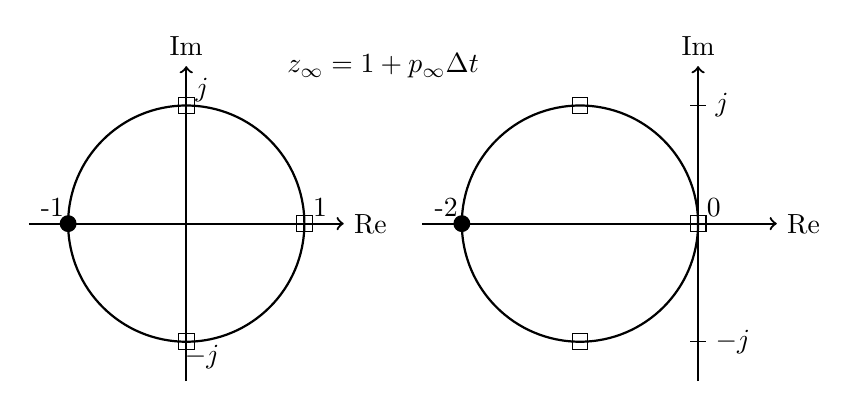
\begin{tikzpicture}
	\node at (2.5,2) {$z_\infty = 1 + p_\infty\Delta t$};

	\draw[thick,->] (-2,0) -- (2,0) node[right]{Re};
	\draw[thick,->] (0,-2) -- (0,2) node[above]{Im};
	\draw[thick] (0,0) circle (1.5);
	\draw (1.4,-0.1) rectangle (1.6,0.1) ++ (.1,.1) node {1};
	\draw (-0.1,1.4) rectangle (0.1,1.6) ++ (.1,.1) node {$j$};
	\filldraw (-1.5,0) circle (0.1) ++ (-.2,.2) node {-1};
	\draw (-0.1,-1.4) rectangle (0.1,-1.6) ++ (.1,-.1) node {$-j$};
	
	\draw[thick,->] (3,0) -- (7.5,0) node[right]{Re};
	\draw[thick,->] (6.5,-2) -- (6.5,2) node[above]{Im};
	\draw[thick] (5,0) circle (1.5);
	\draw (6.4,1.5) -- (6.6,1.5) node[right] {$j$};
	\draw (6.4,-1.5) -- (6.6,-1.5) node[right] {$-j$};
	\draw (6.4,-0.1) rectangle (6.6,0.1) ++ (.1,.1) node {0};
	\draw (4.9,1.4) rectangle (5.1,1.6);
	\filldraw (3.5,0) circle (0.1) ++ (-.2,.2) node {-2};
	\draw (4.9,-1.4) rectangle (5.1,-1.6);
	
\end{tikzpicture} 

\caption{Stabilitätsbereich für den expliziten Euler}
\end{figure}

Somit ist die Wahl von $\Delta t$ aus Stabilitätsgründen eingeschränkt. Bei zu großem $\Delta t$ liegt das Produkt $p_\infty \Delta t$ nicht mehr im Stabilitätsbereicht. Praktisch beim expliziten Euler ist hingegen, dass es keine Stabilität in der rechten Halbebene gibt, es werden also instabile System als instabil detektiert.

Im folgenden noch einmal die Eigenschaften der Verfahren kurz zusammengefasst:

\begin{tabular}{r|c|c|c|c|c}
& explizit/implizit & Schritte & Ordnung & stabil für $\Re{p_\infty} < 0$ & asymptotisch stabil \\ \hline
expliziter Euler & explizit & 1 & 1 & nein & nein \\ \hline
impliziter Euler & implizit & 1 & 1 & ja & ja \\ \hline
Trapez & implizit & 1 & 2 & ja & nein \\ \hline
Gear & implizit & 2 & 2 & ja & ja
\end{tabular}
Zudem haben Einschrittverfahren Vorteile beim Starten, mit Mehrschrittverfahren kann nicht direkt gestartet werden.

\section{Taylor-Verfahren höherer Ordnung}
Die eher im technischen Bereich gängige Schreibweise
\begin{equation}
y(\nu + 1) = y(\nu) + \Delta t T^{(n)}(\nu, y(\nu))
\end{equation}
ist äquivalent zur in der Mathematik üblichen Variante
\begin{equation}
y_{i + 1} = y_i + h T^{(n)} (t_i, y_i)
\end{equation}
mit
\begin{equation}
T^{(n)}(t_i, y_i) = f(t_i, y_i) + \frac{h}{2} f'(t_i, y_i) + \dots + \frac{h^{n - 1}}{n!} f^{(n - 1)}(t_i, y_i)
\end{equation}

Dadurch erhält man einer bessere Genauigkeit, genauer gesagt: $\epsilon O(h^n)$. Nachteilig kann sich allerdings auswirken, dass höhere Ableitungen der Funktion benötigt werden.

\section{Prädiktor-Korrektor-Ansätze}
Die Grundidee dahinter ist ein explizites Verfahren zur Vorhersage des Wertes $y_{i + 1}$ zu nutzen, und diesen Werte nachträglich mithilfe eines weiteren Verfahrens zu verbessern. Dieser Ansatz kann auch iterativ verwendet werden.

Ein Beispiel für so einen Prädiktor-Korrektor-Ansatz ist das Verfahren von Heun, welches auf einem expliziten Euler basiert. Der explizite Euler liefert
\begin{equation}
y_{i + 1}^0 = y_i + h \cdot f(t_i, y_i)
\end{equation}
und daraus berechnet Hoin ein verbessertes
\begin{equation}
y_{i + 1}^1 = f(t_{i + 1}, y_{i + 1}^0) .
\end{equation}

Der iterativer Ansatz dazu wäre dann
\begin{equation}
y_{i + 1}^0 = y_i + h \cdot f(t_i, y_i)
\end{equation}
\begin{equation}
y_{i + 1}^j = y_i^m + h \cdot \frac{f(t, y_i^m) + f(t_{i + 1}, y_{i + 1}^{j - 1}}{2}
\end{equation}

\section{Adams-Bashforth/Adams-Moulton}
Die Grundidee hinter diesen Verfahren beruht darauf $f$ durch ein Interpolationspolynom zu ersetzen.

Ausgangspunkt ist die Differentialgleichung
\begin{equation}
y' = f(t, y)
\end{equation}
wobei $a \le t \le b$ und $y(a) = \alpha$.

Adams-Bashforth und Adams-Moulton sind $m$-schrittige Mehrschrittverfahren, in denen $y_{i + 1}$ ersetzt wird durch 
\begin{equation}
y_{i + 1} = a_{m - 1} y_i + a_{m - 2} y_{i - 1} + \dots + a_0 y_{i + 1 - m} + h \left[ b_m f(t_{i + 1}, y_{i + 1}) + b_{m - 1} f(t_i, y_i) + \dots + b_0 f(t_{i + 1 - m}, y_{i + 1 - m}) \right]
\end{equation}
mit $i = m - 1, m, \dots N - 1$, $h = \frac{b - a}{N}$. Falls $b_n = 0$ spricht man von einem expliziten Verfahren, ansonsten von einem impliziten.

\paragraph{Herleitung}
\begin{equation}
y(t_{i + 1}) = y_{i + 1}
\end{equation}
\begin{equation}
y_{i - 1} - y_i = \int_{t_i}^{t_{i + 1}} y'(t) \diff t = \int_{t_i}^{t_{i + 1}} f(t_i, y(t)) \diff t
\end{equation}
\begin{equation}
y_{i + 1} = y_i + \int_{t_i}^{t_{i + 1}} f(t_i, y(t)) \diff t
\end{equation}
Ersetze $f(t_i, y(t)) $ durch Interpolationspolynom $P(t)$
\begin{equation}
y_{i + 1} \approx y_i + \int_{t_i}^{t_{i + 1}} P(t) \diff t
\end{equation}

Für das Interpolationspolynom bieten sich an
\begin{itemize}
\item Taylor
\item Lagrange
\item Newton'sche Rückwärtsdifferenzen
\end{itemize}

\paragraph{Adams-Bashforth (explizit)}
Die explizite Einschrittvariante ist äquivalent zum expliziten Euler:
\begin{equation}
y_{i + 1} = y_i + h f(t_i, y_i)
\end{equation}
Die Variante mit zwei Schritten lautet
\begin{equation}
y_{i + 1} = y_i + \frac{h}{2} \left[ 3 f(t_i, y_i) - f(t_{i - 1}, y_{i - 1} \right]
\end{equation}
und hat eine quadratisches Fehlerverhalten.

\paragraph{Adams-Moulton (implizit)}
Die Einschrittvariante hiervon ist für $m = 0$ der implizite Euler, für $m = 1$ das Trapezverfahren. Wenn zwei Schritten verwendet werden sieht das Verfahren wie folgt aus
\begin{equation}
y_{i + 1} = y_i + \frac{h}{12} \left[ 5 f(t_{i + 1}, y_{i + 1} + 8 f(t_i, y_i) - f(t_{i - 1}, y_{i - 1}) \right]
\end{equation}
und besitzt ein kubisches Fehlerverhalten.

\section{Ausgleichsrechnung (Approximation, Least Square)}
\textbf{Ziele der Approximation:} ("`curve fitting"')
\begin{itemize}
\item Bestgeeignete Funktion eines bestimmten Typs, um gegebenen Daten anzunähern
\item Für gegebene Funktionen "`bestmögliche"', einfachere Funktionen zu finden. 
\end{itemize}

\textbf{"`Bestmögliche"' Funktion zur Annäherung gegebener Stützpunkte}
\begin{itemize}
\item Gegeben: Wertepaare $(x_i,y_i),\;i=1,\ldots ,m$
\item Annahme: Gerade beschriebt Wertepaare $y = f(x) = ax+b$ 
\end{itemize}

\textbf{Ansätze:} 
\begin{itemize}
\item $E = \sum\limits_{i=1}^m l_i = \sum\limits_{i=1}^m\left[y_i-(ax_i+b)\right]$
\item $E = \sum\limits_{i=1}^m \abs{l_i} = \sum\limits_{i=1}^m\abs{\left[y_i-(ax_i+b)\right]}$
\item Minmax: $\min E_\infty = \min\max\limits_{i=1,\ldots,m}\left\lbrace\abs{y_i-(ax_i+b)}\right\rbrace$
\end{itemize}

\paragraph{Linear Least Squares}
Minimiere: $E_2(a,b) = \sum\limits_{i=1}^m\left(y_i-(ax_i+b)\right)^2$\\
Bestimmung von $a,b$: $\frac{\partial E_2}{\partial a} = 0,\;\frac{\partial E_2}{\partial b} = 0$\\
$\Rightarrow$ Normalengleichung:
\begin{itemize}
\item $a = ...$
\item $b = ...$
\end{itemize}

\paragraph{Polynominale Least Squares}
Approximation durch $P_n(x) = a_nx^n + \ldots + a_1x + a_0$
\begin{equation}
E_2(a_0,a_1,\ldots,a_n)) = \sum\limits_{i=1}^m(y_i - P(x_i)^2) 
\end{equation}
Minimierung $\frac{\partial E_2}{\partial a_i} = 0\Rightarrow n+1$ Normalengleichungen in den $n+1$ Unbekannten $a_0,\ldots,a_n$

\paragraph{Linear Least Squares - Sichtweise Lineare Algebra}
\begin{equation}
\ma{A}_{<m\times n}\cdot\vec{x}_{n} = \vec{b}_{n}\quad,m>n
\end{equation}
Beispiel:
\begin{itemize}
\item $m=2,n=1\quad\begin{bmatrix}
a_1 \\ a_2
\end{bmatrix}\cdot x = \begin{bmatrix}
b_1 \\ b_2
\end{bmatrix}$
\item $m=3,n=2\quad\begin{bmatrix}
a_{11} & a_{12} \\ a_{21} & a_{22} \\ a_{31} & a_{32}
\end{bmatrix}\cdot \begin{bmatrix}
x_1 \\ x_2
\end{bmatrix} = \begin{bmatrix}
b_1 \\ b_2 \\ b_3
\end{bmatrix}$
\end{itemize}

Fehler je Zeile: $e_i = b_i - \vec a_i\cdot \vec x$\\
Vektor der Fehler: $\vec e = \vec b - \ma{A}\cdot \vec x$\\
Summe der Fehlerquadrate: $E_2 = \norm{e}^2 = \norm{\vec b - \ma A\vec x}^2$\\
Gesucht $\hat{\vec x}$, so dass $E_2$ minimiert wird.
\begin{equation}
\ma A\hat{\vec x} = \vec p \quad ; \quad \vec e = \vec b - \vec p
\end{equation}
$\vec p$ ist die Projektion von $\vec b$ in den Spaltenraum von $\col(\ma A)$\\
$\vec e$ steht senkrecht auf den Spaltenraum $\col(\ma A)$
\begin{equation}
\begin{split}
E(x) &= \norm{\vec b - \ma A\vec x}^2 = \norm{\ma A\vec x - \vec b}\\
&= \vec x^T\ma A^T\ma A\vec x - (\ma A\vec x)^T\vec b - \vec b^T\ma A\vec x - \vec b^T\vec b\\
&= \vec x^T\underbrace{\ma A^T\ma A}_{\ma K}\vec x - 2\vec x^T\underbrace{\ma A^T\vec b}_{\vec f} - \vec b^T\vec b\\
&= \vec x^T\ma K\vec x - 2\vec x^T\vec f + \vec b^T\vec b\quad\text{zu minimieren}\\
&= (\vec x-\ma K^{-1}\vec f)^T\ma K(\vec x-\ma K^{-1}ßvec f) - \vec f^T\ma K^{-1}\vec f + \vec b^T\vec b
\end{split}
\end{equation}
Ausdruck kann minimal 0 werden für $\hat{\vec x} = \ma K^{-1}\vec f\Rightarrow$ dort also Minimum vom $E(\vec x)$
\begin{equation}
\begin{split}
E_\text{min} = E(\hat{\vec x}) &= (\vec b - \ma A\hat{\vec x})^T\cdot(\vec b - \ma A\hat{\vec x})\\
&= \vec b^T\vec b - \vec f^T\ma K^{-1}\vec f\\
&= \vec b^T\vec b - \vec b^T\ma A(\ma A^T\ma A)^{-1}\ma A^T\vec b
\end{split}
\end{equation}
$\vec e = \vec b - \ma A\vec x$ steht senkrecht auf $\col(\ma A)\Rightarrow\ma A^T\vec e = \vec 0$\\
\begin{equation}
\Rightarrow \ma A^T(\vec b - \ma A\hat{\vec x}) = 0 \Rightarrow \ma A^T\ma A\hat{\vec x} = \ma A^T\vec b
\end{equation}
$\underbrace{\ma A^T\ma A\hat{\vec x} = \ma A^T\vec b}_{\text{quadratisch, symmetrisch}} \text{ LGS }\Rightarrow\text{ Bestimmung von }\hat{\vec x}$

\textbf{Lösungsverfahren:}
\begin{itemize}
\item Gauß LU: OK, aber $\cond(\ma A^T\ma A) = \cond(\ma A)^2\Rightarrow$ Problematisch, wenn $\ma A$ schlecht konditioniert
\item Orthogonalzerlegung
\end{itemize}

\subsection{QR-Zerlegung}
\[\ma A = \ma Q\ma R \text{ mit }\begin{cases}
\ma A & \in \R^{n\times n}\\
\ma Q & \in \R^{n\times n} \text{orthogonale Matrix} (\ma Q^T = \ma Q^{-1})\\
\ma R & \in \R^{n\times n} \text{rechte obere Dreiecksmatrix}
\end{cases}\]
Damit:
\begin{equation}
\begin{split}
\ma A\vec x &= \vec b\\
\ma A^T\ma A\vec x &= \ma A^T\vec b\\
(\ma Q\ma R)^T\ma Q\ma R\vec x &= (\ma Q\ma R)^T\vec b\\
\ma R^T\underbrace{\ma Q^T\ma Q}_{\ma 0}\ma R\vec x &= \ma R^T\ma Q^T\vec b\\
\ma R^T\ma R\vec x &= \ma R^T\ma Q^T\vec b\quad\vert\cdot{\ma R^{-1}}^{-1}\\
\ma R\vec x &= \ma Q^T\vec b\Rightarrow \text{simple Rücksubstitution}
\end{split}
\end{equation}
OK, wie bestimme ich nun $\ma Q,\ma R$?

\textbf{3 wesentliche Ansätze:}
\begin{itemize}
\item Gram-Schmidt
\item Hausholder-Transformation
\item Givens-Rotation
\end{itemize}

\paragraph{Givens-Rotation}
auch bekannt unter der Bezeichung Jacobi-Rotation \\
Eine Rotation ist gegeben durch
\begin{equation}
	\ma G(l, k, \Theta) = 
	\begin{bmatrix}
		1 & 0 & \hdots & \hdots & \hdots & \hdots & \hdots & 0 \\
		0 & 1 & & & & & & 0 \\
		\vdots & & c & & & -s & & \vdots \\
		\vdots & & & & & & & \vdots \\
		\vdots & & -s & & & c & & \vdots \\ 
		\vdots & & & & & & 1 & 0 \\ 
		0 & \hdots & \hdots & \hdots & \hdots & \hdots & 0 & 1 
	\end{bmatrix}
\end{equation}
wobei $c = \cos \Theta$, $s = \sin \Theta$. Komponentenweise $\ma G(l, k, \Theta) =  (g_{i,j}(l, k, \Theta))$ dargestellt ergibt das
\begin{equation}
	g_{i,j} = 
	\begin{cases} 
		\cos \Theta & \text{für } i = l, j = l \vee i = k, j = k \\
		\sin \Theta & \text{für } i = l, j = k \\
		- \sin \Theta & \text{für } i = k, j = l \\
		1 & \text{für } i = j \text{ außer } i, j = l, k \\
		0 & \text{sonst}
	\end{cases}
\end{equation}
Damit bedeutet $\ma G \cdot \vec x$ bzw. $\ma G^T \cdot \vec x$ eine Drehung des Vektors $\vec x$ um $\pm \Theta$ in der $(l, k)$-Ebene. Die Hauptanwendung hierfür ist ein iteratives Vorgehen um Nulleinträge in Matrizen oder Vektoren zu erreichen. Desweiteren ist $\ma G \ma G^T = \ma I$ und somit die Rotationsmatrix $\ma G$ orthogonal.
\begin{equation}
	\begin{pmatrix}
		c & s \\
		-s & c
	\end{pmatrix} 
	\begin{pmatrix}
		c & -s \\
		s & c
	\end{pmatrix} = 
	\begin{pmatrix}
		c^2 + s^2 & 0 \\
		0 & c^2 + s^2
	\end{pmatrix} =
	\begin{pmatrix}
		1 & 0 \\
		0 & 1
	\end{pmatrix} 
\end{equation}
Damit gilt
\begin{equation}
	\ma G_r \ma G_{r - 1} \cdot \ldots \cdot \ma G_2 \ma G_1 \ma A = \ma R
\end{equation}
\begin{equation}
	\ma A = \ma G^T \ma R = \ma Q^T \ma R
\end{equation}
Die Frage ist nun, wie $\Theta$ gewählt werden muss. Hierfür genügt die Betrachtung einer zweidimensionalen Struktur
\begin{equation}
	\begin{pmatrix}
		c & s \\
		-s & c
	\end{pmatrix} 
	\begin{pmatrix}
		x_l \\
		x_k
	\end{pmatrix} = 
	\begin{pmatrix}
		r \\
		0
	\end{pmatrix}
\end{equation}
Daraus kann gefolgert werden, dass
\begin{equation}
	s = c \frac{x_k}{x_l}
\end{equation}
und aus
\begin{equation}
	c^2 + s^2 = 1
\end{equation}
\begin{equation}
	c = \sqrt{1 - s^2} = \sqrt{\frac{x_l^2 - c^2 x_k^2}{x_l^2}}
\end{equation}
\begin{equation}
	c^2 x_l^2 = x_l^2 - c^2 - x_k^2
\end{equation}
\begin{equation}
	c = \pm \frac{x_l}{\sqrt{x_l^2 + x_k^2}}
\end{equation}
Das ganze an dem Beispiel
\begin{equation}
	\ma A = 
	\begin{pmatrix}
		3 & 1 & 0 \\
		1 & 3 & 1 \\
		0 & 1 & 3	
	\end{pmatrix}
\end{equation}
führt über
\begin{equation}
	\ma G = 
	\begin{pmatrix}
		c & s & 0 \\
		-s & c & 1 \\
		0 & 0 & 1	
	\end{pmatrix}
\end{equation}
zu
\begin{equation}
	\ma G \ma A =
	\begin{pmatrix}
		\sqrt{10} & 6/\sqrt{10} & 1/\sqrt{10} \\
		0 & 3/\sqrt{10} & 3/\sqrt{10} \\
		0 & 1 & 3	
	\end{pmatrix}
\end{equation}